\documentclass[12pt,a4paper]{ctexart}

\usepackage{../../Styles/mystyle-report}

\graphicspath{{./image/}}% 指定图片目录，后续可以直接使用图片文件名。

% 去掉交叉引用方框
\hypersetup{
colorlinks=true,    % 启用彩色链接（替代方框）
linkcolor=black,    % 图表/章节引用 纯黑色（无框）
citecolor=black,    % 文献引用 纯黑色
urlcolor=blue       % 网址保留蓝色（美观）
}

% 重定义section左对齐
\makeatletter
% 重定义 \section 命令（一级标题）
\renewcommand{\section}{\@startsection{section}{1}{\z@}%
% 参数4：标题 上方 的空白距离（负数是固定写法）
{-0ex \@plus -1ex \@minus -.2ex}%
% 参数5：标题 下方 的空白距离（标题和正文之间的距离）
{2.3ex \@plus.2ex}%
% 参数6：标题样式：默认字体+大号+加粗+左对齐
{\normalfont\Large\bfseries\raggedright}}
% 关闭内部命令权限（成对使用）加\raggedright实现左对齐
\makeatother

% 设置页眉页脚
\pagestyle{fancy}  % 使用 fancy 页眉页脚样式
\fancyhf{}  % 清除所有页眉页脚
\renewcommand{\headrulewidth}{0pt}  % 去掉页眉横线
\fancyfoot[C]{\thepage}  % 页码放在页脚中间

% 定义标题页样式（无页码）
\fancypagestyle{titlepage}{
\fancyhf{}  % 清除所有页眉页脚
\renewcommand{\headrulewidth}{0pt}  % 去掉页眉横线
\renewcommand{\footrulewidth}{0pt}  % 去掉页脚横线
}

% 标题、作者信息
% \title{\heiti 25-26-2学期时间序列分析实训课程实验报告}
% \date{\today}
% \author{\textbf{姓名：\underline{\quad 邹文杰 \quad} \quad 序号：\underline{\quad 80 \quad}}}

\begin{document}

\thispagestyle{empty}  % 去掉了第一页页码

\vspace*{\fill}  % 顶部自动填充空白（垂直居中）
\begin{center}
\heiti \Huge 25-26-2 学期时间序列分析实训课程实验报告(一) \\[1.8cm]

% 日期放在上方
\Large 2026 年 4 月 21 日 \\[1.2cm]

% 姓名+序号放在下方
\Large 姓名：\underline{\quad 邹文杰 \quad} \quad\quad 序号：\underline{\quad 80 \quad}
\end{center}
\vfill  % 底部自动填充空白（垂直居中）

\newpage

\section{数据集与数据来源}

\begin{itemize}
\item 数据集：中证2000指数（932000）
\item 分析变量：中证2000股票开盘数据（open）
\item 数据来源：\url{https://www.csindex.com.cn/#/indices/family/detail?indexCode=932000}
\end{itemize}

对开盘数据(open)取对数，记为对数开盘价序列(ln\_open),其时序图如图~\ref{fig:log_open}所示。
\begin{figure}[H]
\centering
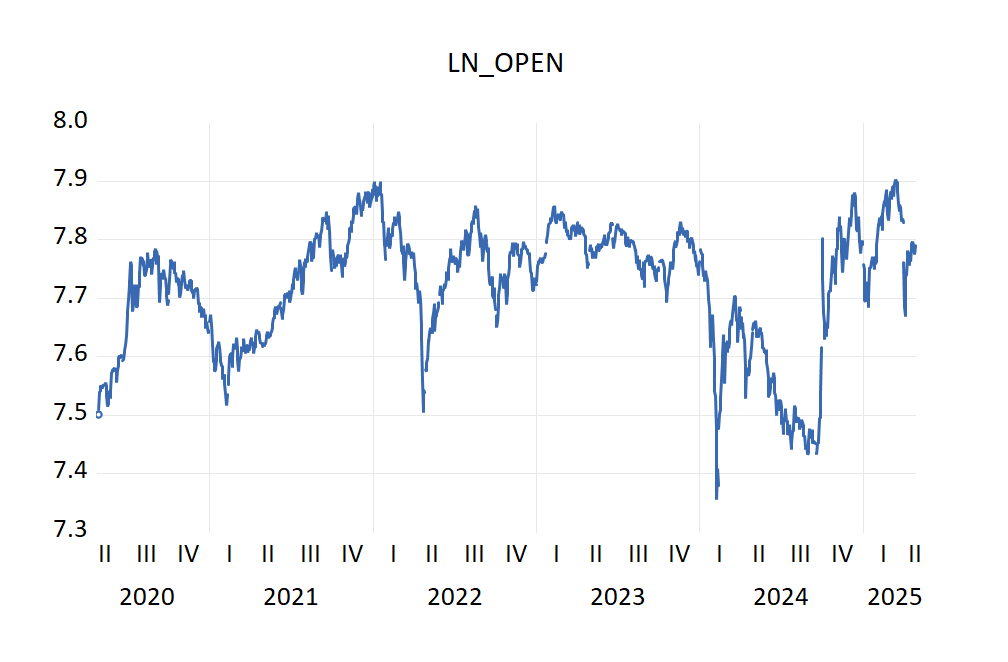
\includegraphics[width=\columnwidth]{log_open.png}
\caption{中证2000指数开盘价对数序列时序图}
\label{fig:log_open}
\end{figure}

\section{时间序列平稳性和非白噪声检验}

对对数开盘价序列(ln\_open)进行单位根检验（ADF检验），分别采用三种模型：无截距无趋势（右下）、仅含截距（左侧）、含截距+线性趋势（右上），结果如图\ref{fig:adf_test}所示。
\begin{figure}[H]
\centering
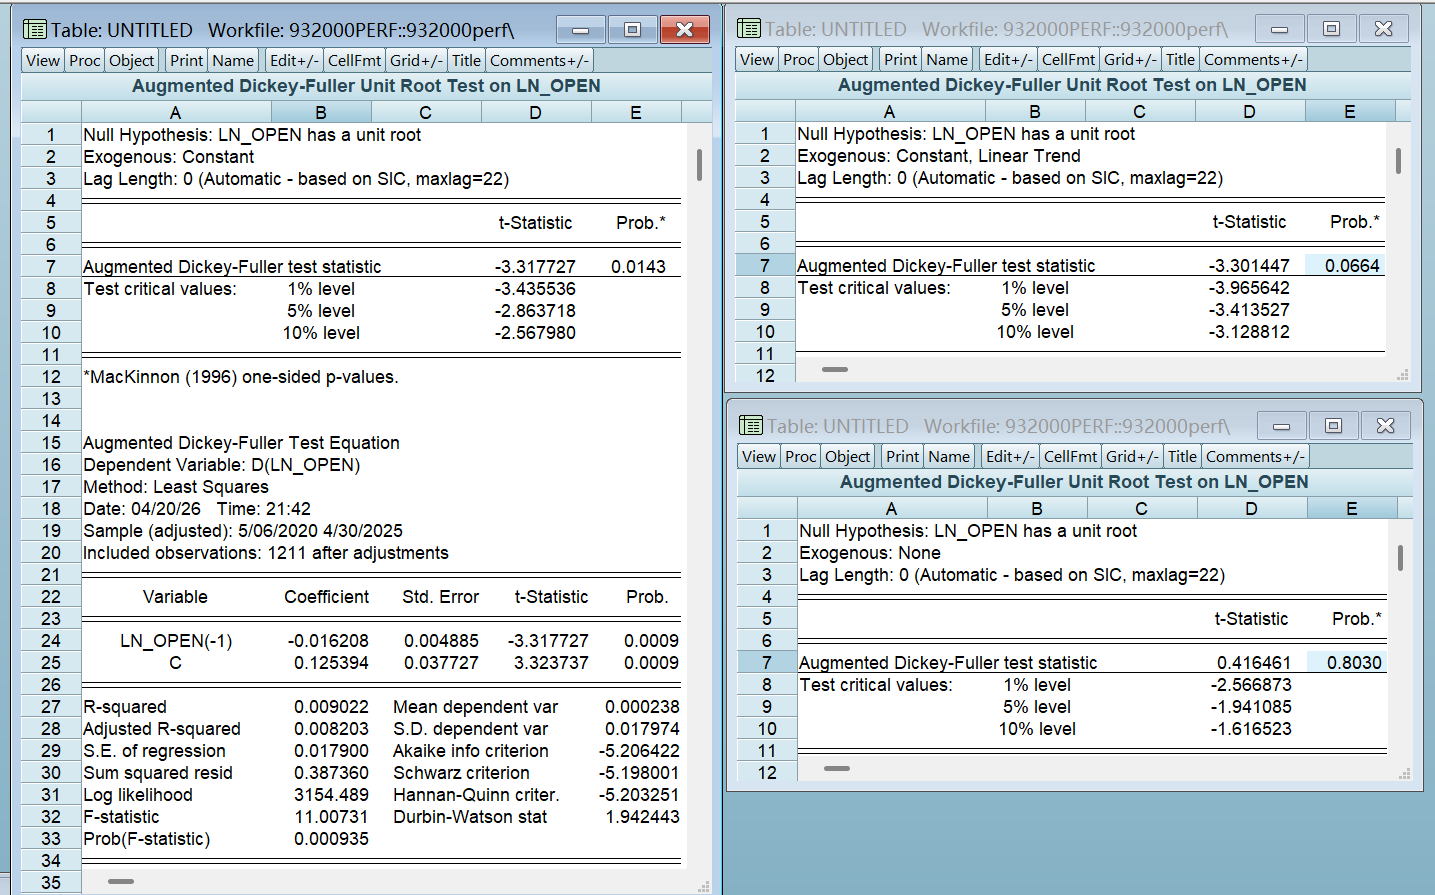
\includegraphics[width=\columnwidth]{adf_test.png}
\caption{对数开盘价序列(ln\_open)的单位根检验图}
\label{fig:adf_test}
\end{figure}
由图~\ref{fig:adf_test}可知,三种模型中，仅含截距模型的P值为0.0143<0.05，在5\%显著性水平下拒绝单位根原假设；含截距+线性趋势模型的P值为0.0664>0.05，无截距无趋势模型的P值为0.8030>0.05，均无法拒绝原假设。这说明，仅含截距模型已证明序列在5\%水平下平稳，因此，后续建模选择\textbf{仅含截距}的模型形式。

对数开盘价序列(ln\_open)的白噪声检验如图~\ref{fig:acf_pacf}所示。
\begin{figure}[H]
\centering
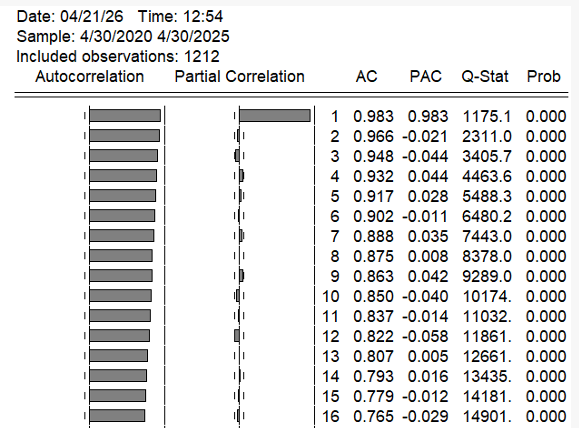
\includegraphics[width=\columnwidth]{acf_pacf.png}
\caption{序列自相关(AC)、偏自相关(PAC)和白噪声检验部分图}
\label{fig:acf_pacf}
\end{figure}
由图~\ref{fig:acf_pacf}可知，对数开盘价序列(ln\_open)的白噪声检验：
\begin{itemize}
\item 序列的自相关系数（AC）在滞后1阶为0.983，随着滞后阶数增加呈缓慢衰减的趋势，滞后36阶仍为0.494（图~\ref{fig:acf_pacf}只展示了滞后16阶），始终位于置信区间外，说明序列存在显著的长期正自相关性，不满足白噪声序列的无自相关假设。

\item 各滞后阶数对应的Q统计量p值均为0.000，小于0.05的显著性水平，强烈拒绝序列为白噪声的原假设，进一步说明序列存在显著的序列相关性，可以构建时间序列模型进行拟合。
\end{itemize}

\section{样本的自相关和偏自相关函数检验}

对数开盘价序列(ln\_open)的自相关与偏自相关图同样如图~\ref{fig:acf_pacf}所示。结果分析如下：
\begin{itemize}
\item 自相关函数（ACF）特征：序列的自相关系数（AC）随着滞后阶数增加呈缓慢衰减的\textbf{拖尾}特征。

\item 偏自相关函数（PACF）特征：偏自相关系数（PAC）仅在滞后1阶显著不为零（0.983），滞后2阶及以后的PAC值均迅速落入置信区间内，呈现\textbf{1阶截尾}特征，说明序列的偏自相关结构可由一阶自回归项充分刻画。
\end{itemize}


\section{模型识别、模型定阶与参数估计}

由图~\ref{fig:acf_pacf}和对数开盘价序列(ln\_open)的自相关/偏自相关特征可知，其ACF呈拖尾特征，PACF呈1阶截尾特征，可选择AR模型进行建模。对对数开盘价序列(ln\_open)分别建立AR(1)、AR(2)、AR(3)模型，如图~\ref{fig:AR123}所示。
\begin{figure}[H]
\centering
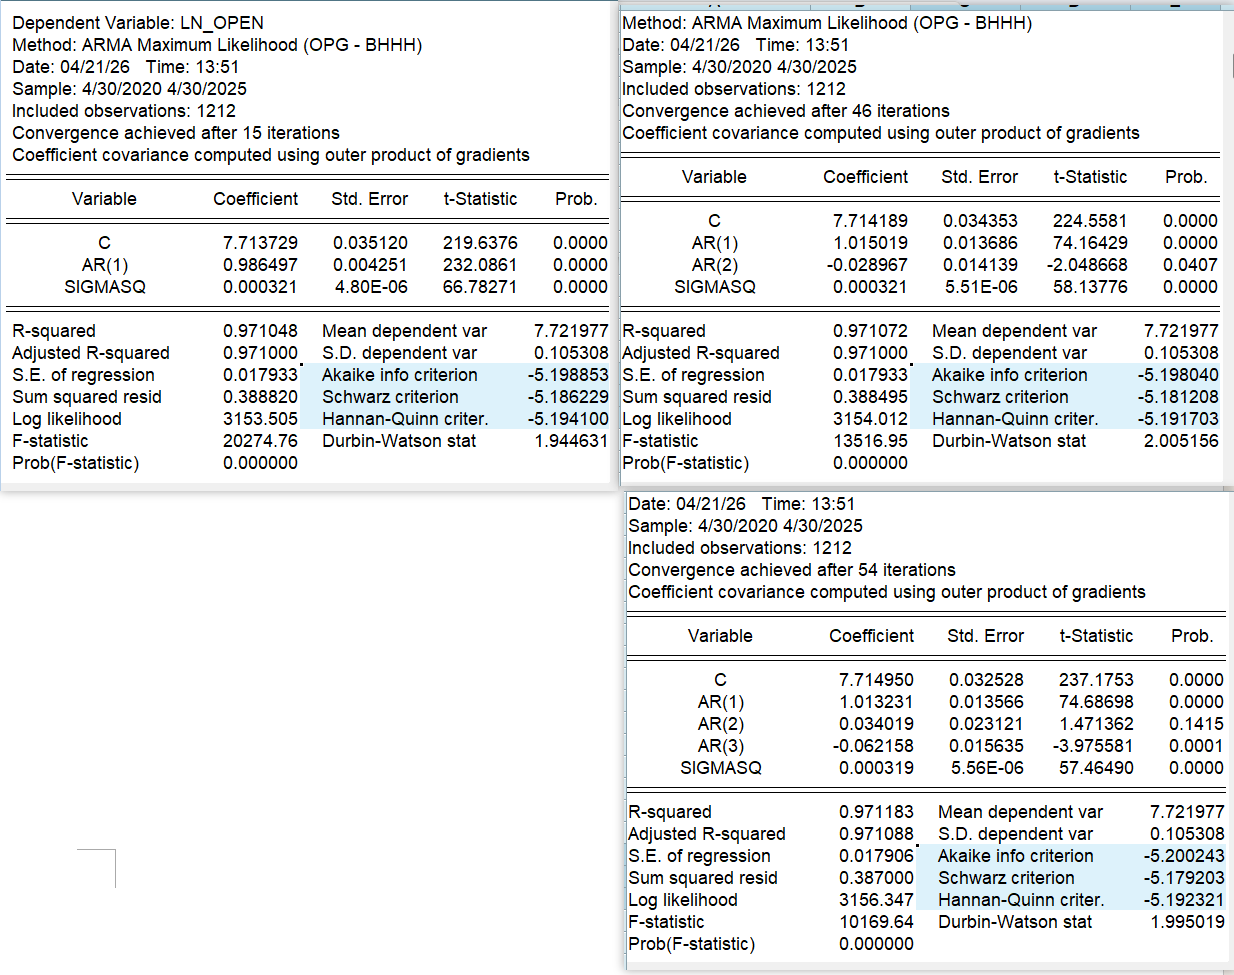
\includegraphics[width=\columnwidth]{AR123.png}
\caption{对数开盘价序列(ln\_open)的AR(1)、AR(2)、AR(3)模型结果图}
\label{fig:AR123}
\end{figure}
整理图~\ref{fig:AR123}中AR(1)、AR(2)、AR(3)的AIC/SC/HQ值如表~\ref{table:不同阶数AR模型的信息准则对比}所示：
\begin{table}[h!]
\centering
\caption{不同阶数AR模型的信息准则对比}
\label{table:不同阶数AR模型的信息准则对比}
\vspace{0.2cm}
\begin{tabular}{lccc}
\hline
模型 & AIC准则 & SC准则 & HQ准则 \\
\hline
AR(1) & -5.1989 & -5.1862 & -5.1941 \\
AR(2) & -5.1980 & -5.1812 & -5.1917 \\
AR(3) & -5.2002 & -5.1792 & -5.1923 \\
\hline
\end{tabular}
\end{table}

根据AIC/SC/HQ准则，AR(1)模型效果最优。对数开盘价序列(ln\_open)的AR(1)模型具体结果图如图~\ref{fig:AR1}所示。
\begin{figure}[H]
\centering
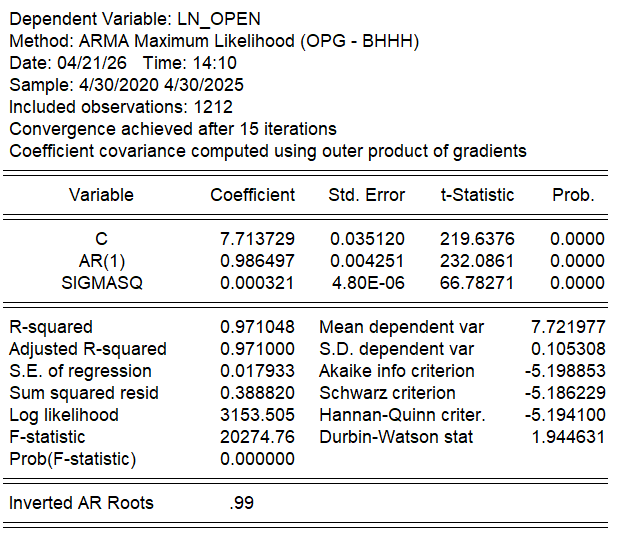
\includegraphics[width=\columnwidth]{AR1.png}
\caption{对数开盘价序列(ln\_open)的AR(1)、AR(2)、AR(3)模型结果}
\label{fig:AR1}
\end{figure}
由图~\ref{fig:AR1}可知，AR(1)模型参数估计均通过显著性检验，常数项$c=7.7137$（$p=0.0000$），说明序列的均值水平显著不为0；一阶自回归系数$\phi_1=0.9865$（$p=0.0000$），说明序列存在极强的一阶正自相关性。模型拟合优度$R^2=0.9710$，表明模型可解释序列97.1\%的变异，拟合效果极佳。

综上可知,对数开盘价序列(ln\_open)的AR(1)模型形式为：
\begin{align*}
\widehat{\mathrm{LN}\_\mathrm{OPEN}}_t&=c+\phi _1\cdot \mathrm{LN}\_\mathrm{OPEN}_{t-1}+\varepsilon _t
\\
&=7.7137+0.9865\cdot \mathrm{LN}\_\mathrm{OPEN}_{t-1}+\varepsilon _t,
\end{align*}
其中，$c$ 为常数项，$\phi_1$ 为一阶自回归系数，$\varepsilon_t$ 为白噪声误差项。


\section{模型适应性检验}

对AR(1)模型的残差序列进行白噪声检验，检验结果如图~\ref{fig:AR1Q}所示。
\begin{figure}[H]
\centering
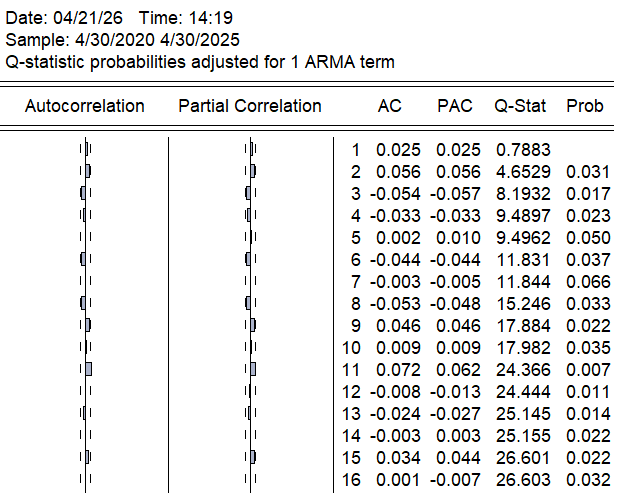
\includegraphics[width=\columnwidth]{AR1Q.png}
\caption{对数开盘价序列(ln\_open)的AR(1)模型适应性检验部分图}
\label{fig:AR1Q}
\end{figure}
由图~\ref{fig:AR1Q}的AR(1)模型适应性检验结果可知：
\begin{itemize}
\item 残差序列的自相关（AC）与偏自相关（PAC）系数数值整体较小，各滞后阶数的残差自相关系数与偏自相关系数大部分都落入置信区间内，无显著的序列相关性。

\item Ljung-Box Q检验结果显示，滞后2阶及以后的大部分滞后阶数的伴随概率（Prob）均小于0.05的显著性水平（如滞后2阶Prob=0.031、滞后3阶Prob=0.017、滞后11阶Prob=0.007等），仅少数滞后阶数的p值大于0.05。
这说明，大部分滞后阶数拒绝原假设，即AR(1)模型的残差仍存在显著的序列相关性，未通过适应性检验。
\end{itemize}



\section{模型优化}

对对数开盘价序列(ln\_open)分别建立ARMA(1,1)、ARMA(1,2)、ARMA(1,3)模型，如图~\ref{fig:ARMA123}所示。
\begin{figure}[H]
\centering
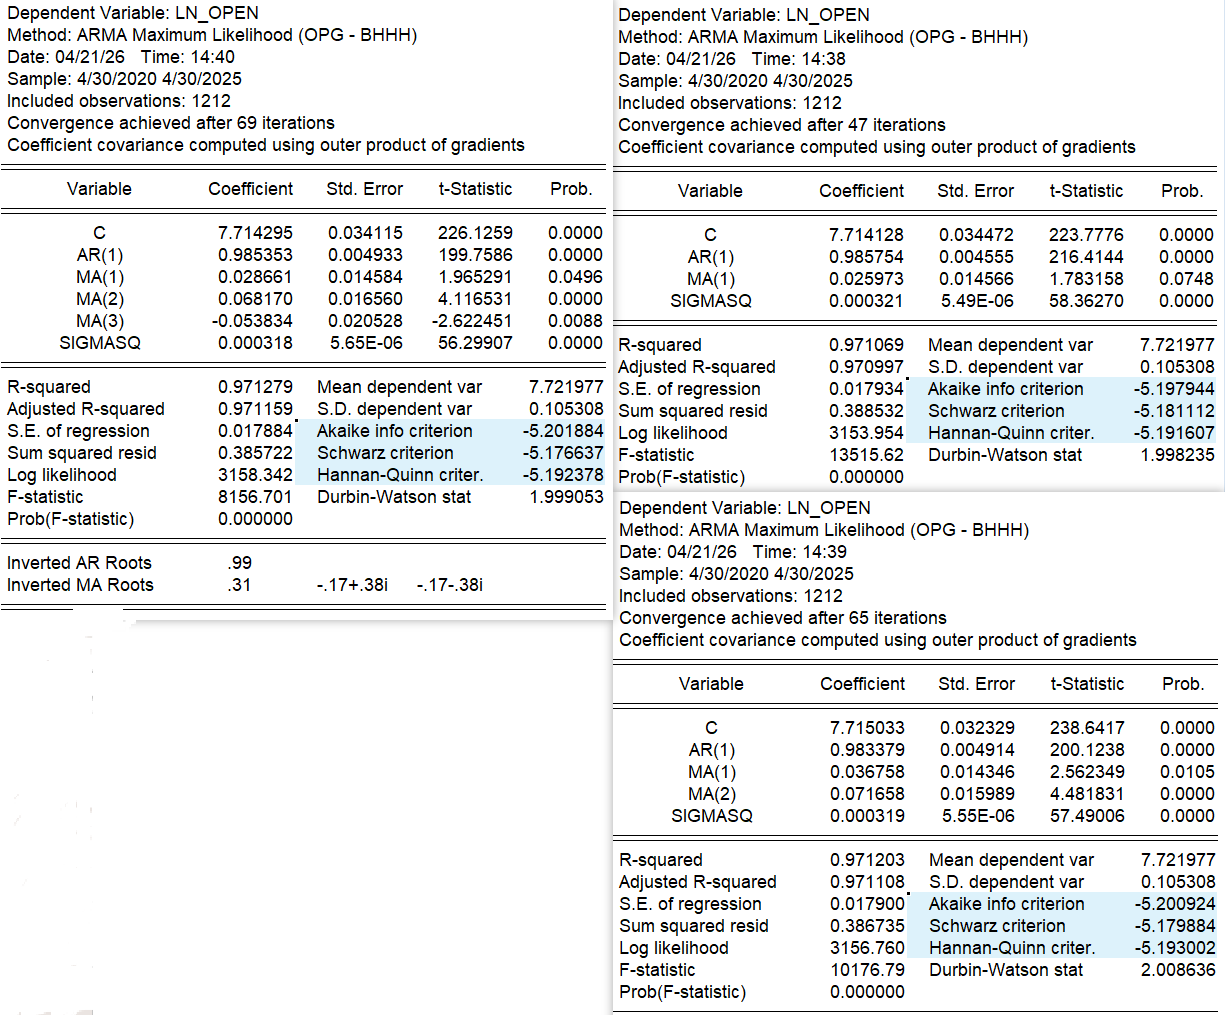
\includegraphics[width=\columnwidth]{ARMA123.png}
\caption{ARMA(1,1)、ARMA(1,2)、ARMA(1,3)模型结果图}
\label{fig:ARMA123}
\end{figure}
整理图~\ref{fig:ARMA123}中ARMA(1,1)、ARMA(1,2)、ARMA(1,3)的AIC/SC/HQ值如表~\ref{table:不同阶数ARMA模型的信息准则对比}所示：
\begin{table}[h!]
\centering
\caption{不同阶数ARMA模型的信息准则对比}
\label{table:不同阶数ARMA模型的信息准则对比}
\vspace{0.2cm}
\begin{tabular}{lccc}
\hline
模型 & AIC准则 & SC准则 & HQ准则 \\
\hline
ARMA(1,1) & -5.1979 & -5.1812 & -5.1916 \\
ARMA(1,2) & -5.2009 & -5.1799 & -5.1930 \\
ARMA(1,3) & -5.2019 & -5.1766 & -5.1924 \\
\hline
\end{tabular}
\end{table}

根据AIC/SC/HQ准则和各模型的自回归系数的P值可知，ARMA(1,3)、ARMA(1,2)模型的AIC/SC/HQ值相近，但ARMA(1,2)有一个自回归系数P值大于0.05，而ARMA(1,3)的自回归系数均小于0.05，故选择ARMA(1,3)模型建模。对数开盘价序列(ln\_open)的ARMA(1,3)模型具体结果图如图~\ref{fig:ARMA2}所示。
\begin{figure}[H]
\centering
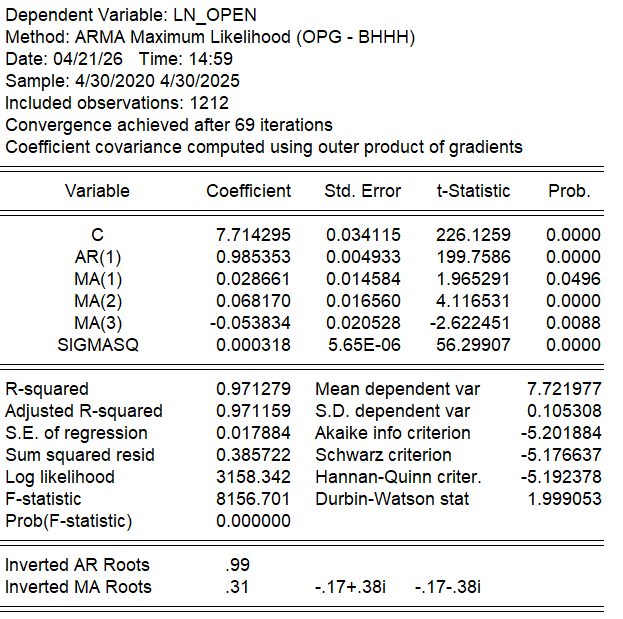
\includegraphics[width=\columnwidth]{ARMA2.png}
\caption{对数开盘价序列(ln\_open)的ARMA(1,3)模型结果图}
\label{fig:ARMA2}
\end{figure}
由图~\ref{fig:ARMA2}可知，模型拟合优度$R^2=0.971279$，表明模型可解释序列97.1279\%的变异，拟合效果极佳。ARMA(1,3) 模型的具体估计形式为：
\begin{align*}
&\widehat{\mathrm{LN}\_\mathrm{OPEN}}_t=c+\phi _1\cdot \mathrm{LN}\_\mathrm{OPEN}_{t-1}+\theta _1\cdot \hat{\varepsilon}_{t-1}+\theta _2\cdot \hat{\varepsilon}_{t-2}-\theta _3\cdot \hat{\varepsilon}_{t-3}+\hat{\varepsilon}_t
\\
&=7.7143+0.9854\cdot \mathrm{LN}\_\mathrm{OPEN}_{t-1}+0.0287\cdot \hat{\varepsilon}_{t-1}+0.0682\cdot \hat{\varepsilon}_{t-2}-0.0538\cdot \hat{\varepsilon}_{t-3}+\hat{\varepsilon}_t,
\end{align*}
其中，$c$为常数项，$\phi_1$为一阶自回归系数，$\theta_1$为一阶移动平均系数，$\theta_2$为二阶移动平均系数，$\theta_3$为三阶移动平均系数，$\hat{\varepsilon}_t$ 为模型残差项，服从均值为0、方差为 $\sigma^2=0.000318$ 的白噪声分布。

再对ARMA(1,3)模型的残差序列进行白噪声检验，检验结果如图~\ref{fig:ARMA2Q}所示。
\begin{figure}[H]
\centering
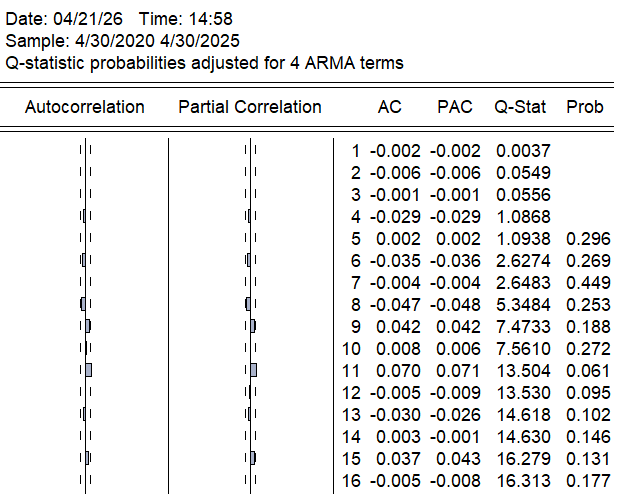
\includegraphics[width=\columnwidth]{ARMAQ2.png}
\caption{对数开盘价序列(ln\_open)的ARMA(1,3)模型适应性检验部分图}
\label{fig:ARMA2Q}
\end{figure}
由图~\ref{fig:ARMA2Q}的ARMA(1,3)模型适应性检验结果可知：
\begin{itemize}
\item 残差序列的自相关（AC）与偏自相关（PAC）系数数值整体较小，各滞后阶数的残差自相关系数与偏自相关系数均落入置信区间内，无显著的序列相关性。

\item Ljung-Box Q检验结果显示，滞后5阶及以后的所有滞后阶数的伴随概率（Prob）均大于0.05的显著性水平（如滞后5阶Prob=0.296、滞后7阶Prob=0.449、滞后11阶Prob=0.061、滞后16阶Prob=0.177等），无显著低于0.05的情况。
这说明，无法拒绝“残差序列无自相关（即残差为白噪声）”的原假设，当前模型的残差不存在显著的序列相关性，通过适应性检验，模型有效。
\end{itemize}




\end{document}